\section{Abstractions}
\label{sec-abs}

\begin{figure}[ht!]
\centerline{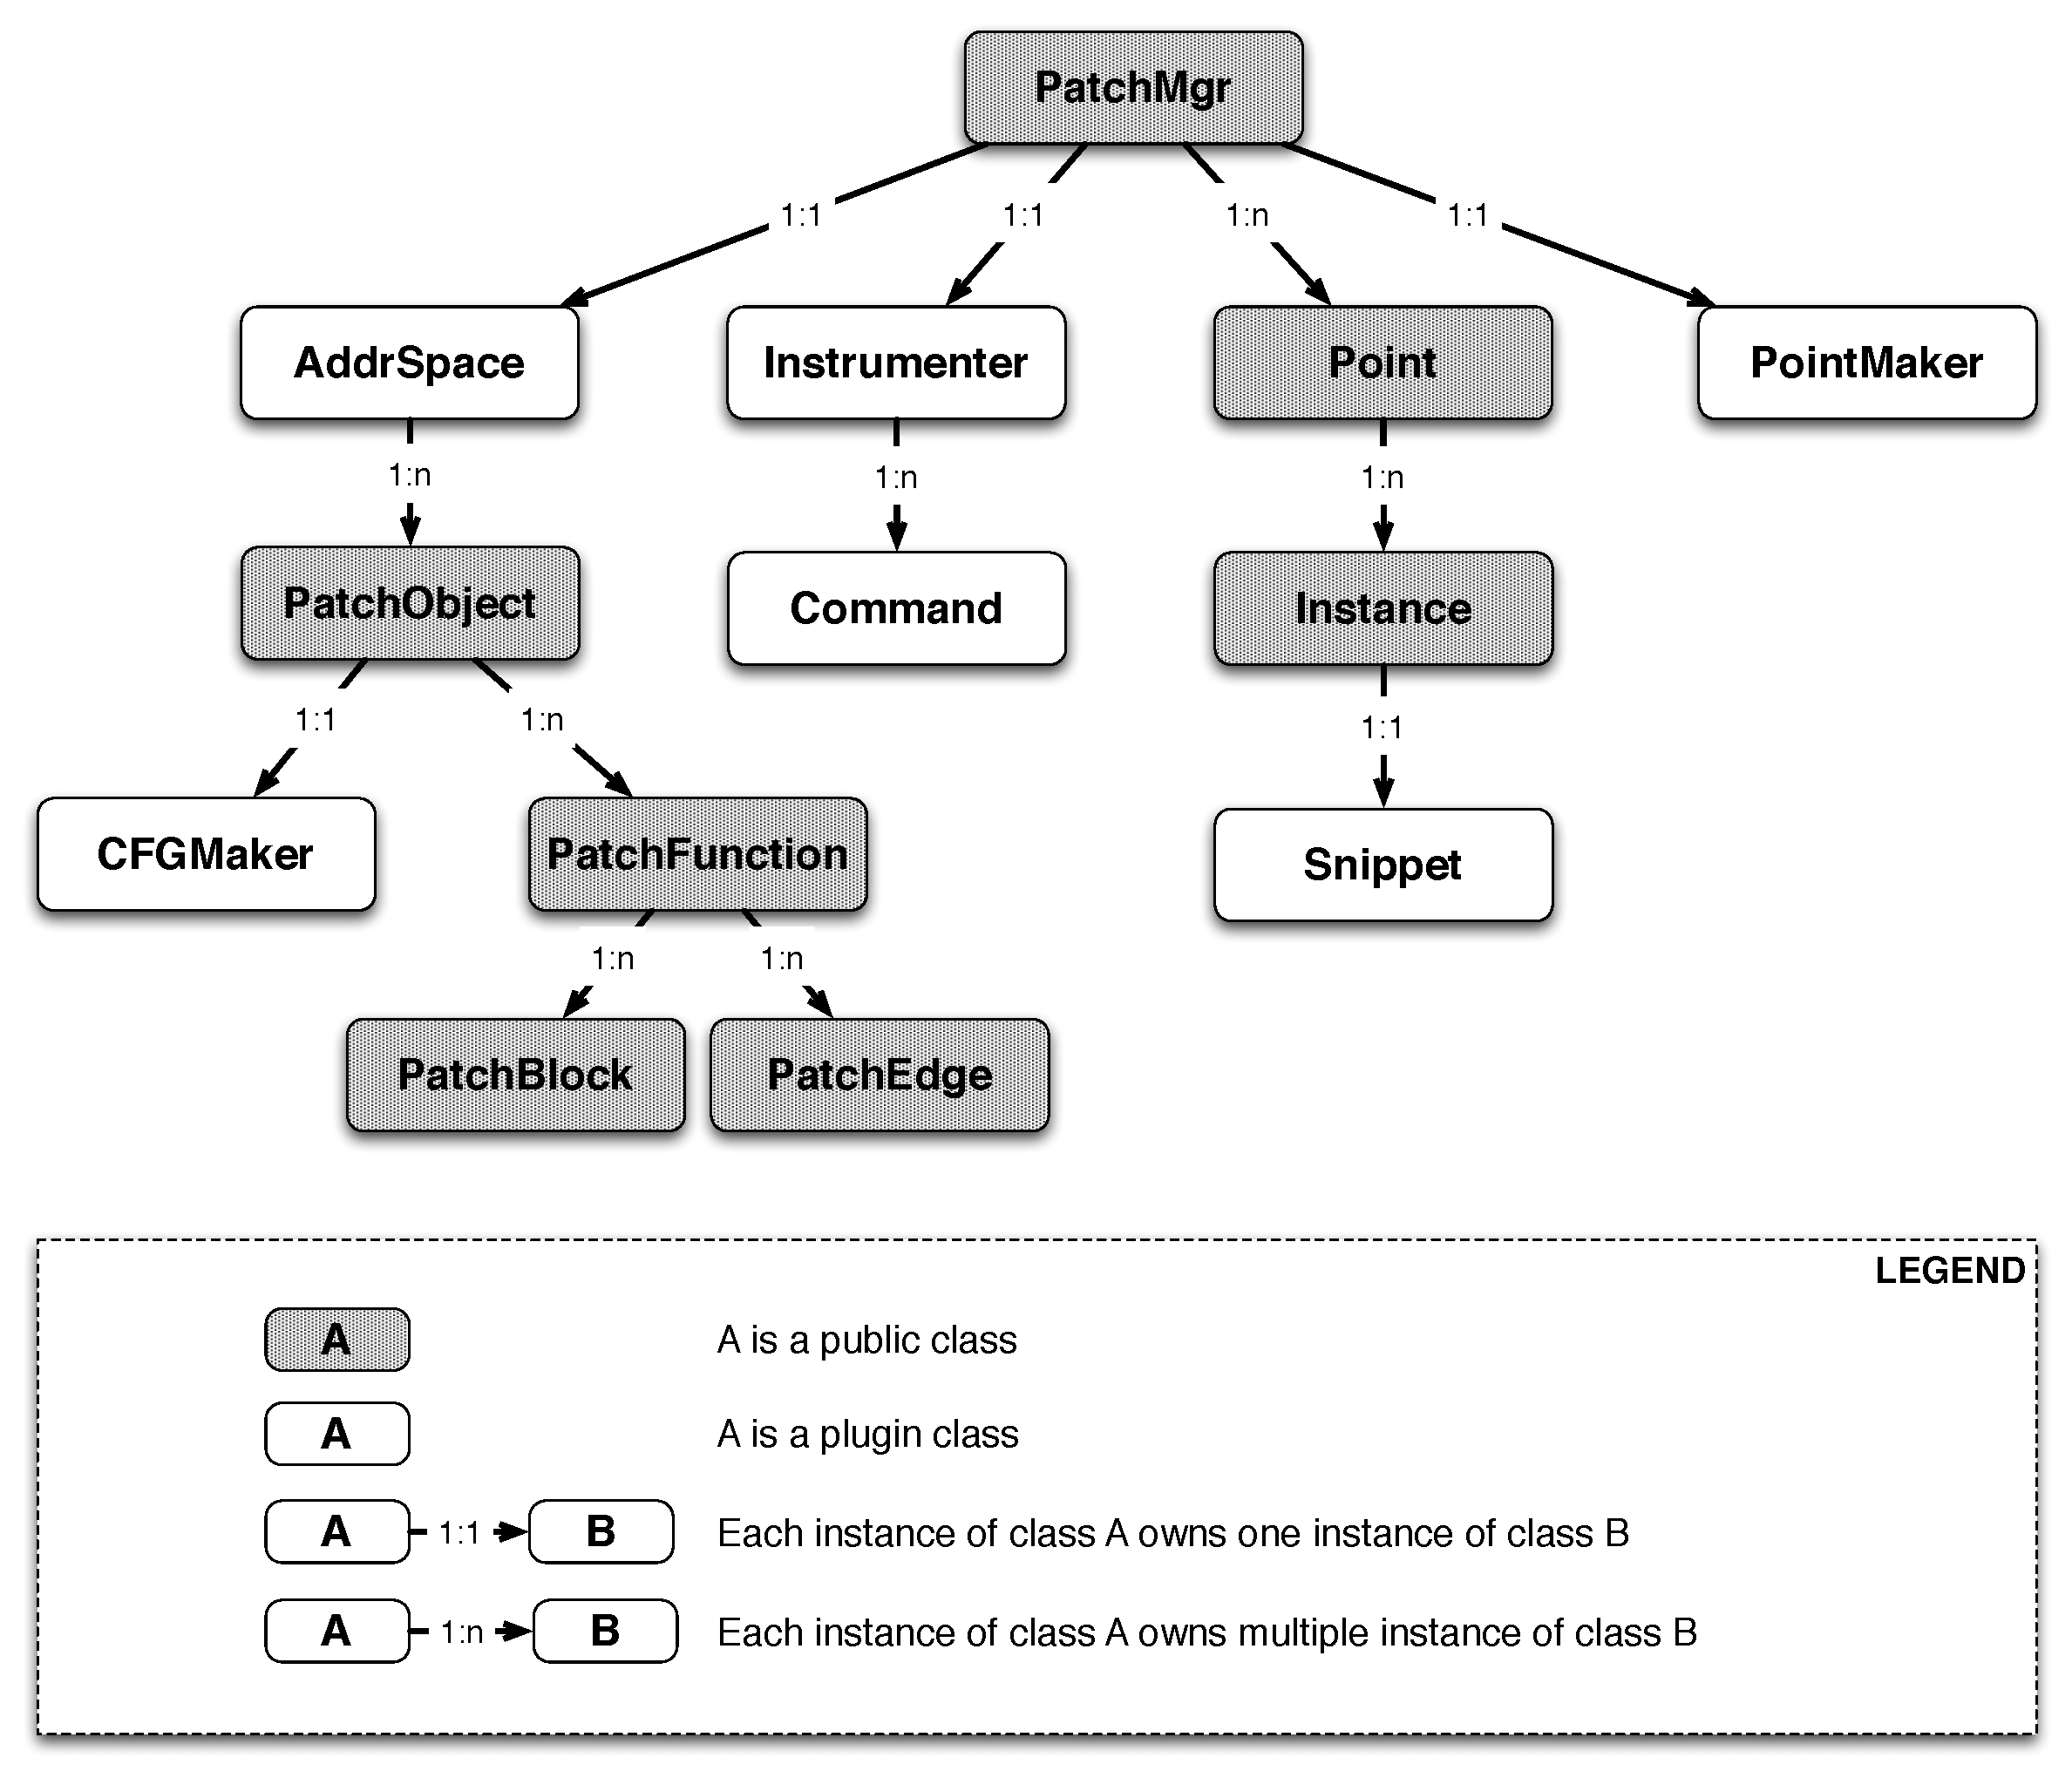
\includegraphics[width=0.85\textwidth]{./figure/abstraction/img.pdf}}
\caption{\label{fig:abs}Object Ownership}
\end{figure}


PatchAPI contains two interfaces: the public interface and the plugin interface.
The public interface is used to find instrumentation points, insert or delete
code snippets, and register plugins provided by programmers. The plugin
interface is used to customize different aspects in the binary code patching.
PatchAPI provides a set of default plugins for first party code patching, which
is easy to extend to meet different requirements in practice.

Figure \ref{fig:abs} shows the ownership hierarchy for PatchAPI's classes.
Ownership is a ``contains'' relationship. If one class owns another, then
instances of the owner class maintain exactly one or possibly more than one
instances of the other, which depends on whether the relationship is a ``1:1''
or a ``1:n'' relationship. In Figure \ref{fig:abs}, for example, each PatchMgr
instance contains exactly one instance of a AddrSpace object, while a PatchMgr
instance may contains more than one instances of a Point object.

The remainder of this section briefly describes the classes that make up
PatchAPI's two interfaces. For more details, see the class descriptions in
Section~\ref{sec-public-api} and Section~\ref{sec-plugin-api}.

\subsection{Public Interface}
\label{sec-2.1}

PatchMgr, Point, and Snippet are used to perform the main process of binary code
patching: 1) find some \textbf{Point}; 2) insert or delete \textbf{Snippet} at some \textbf{Point}.
\begin{itemize}
\item \emph{PatchMgr} - The PatchMgr class is the top-level class for finding
    instrumentation \textbf{Points}, inserting or deleting \textbf{Snippets}, and registering
    user-provided plugins.
\item \emph{Point} - The Point class represents a location on the CFG that acts as a
    container of inserted snippet \textbf{Instances}. Points of different types are
    distinct even the underlying code relocation and generation engine happens
    to put instrumentation from them at the same place.
\item \emph{Instance} - The Instance class is a representation of a particular snippet
    inserted at a particular point.
\item \emph{PatchObject} - The PatchObject class is a wrapper of ParseAPI's CodeObject
    class, which represents an individual binary code object, such as an
    executable or a library.
\item \emph{PatchFunction} - The PatchFunction class is a wrapper of ParseAPI's
    Function class, which represents a function.
\item \emph{PatchBlock} - The PatchBlock class is a wrapper of ParseAPI's Block class,
    which represents a basic block.
\item \emph{PatchEdge} - The PatchEdge class is a wrapper of ParseAPI's Edge class,
    which join two basic blocks in the CFG, indicating the type of control flow
    transfer instruction that joins the basic blocks to each other.
\end{itemize}
\subsection{Plugin Interface}
\label{sec-2.2}

The address space abstraction determines whether the code patching is 1st party,
3rd party or binary rewriting.
\begin{itemize}
\item \emph{AddrSpace} - The AddrSpace class represents the address space of a
  \textbf{Mutatee} (a program that is instrumented), where it contains a
  collection of \textbf{PatchObjects} that represent shared libraries or a
  binary executable. In addition, programmers implement some memory management
  interfaces in the AddrSpace class to determines the type of the code patching
  - 1st party, 3rd party, or binary rewriting.
\end{itemize}
Programmers can decide the representation of a \textbf{Snippet}, for example, the
representation can be in high level language (e.g., C or C++), or can simply be
in binary code (e.g., 0s and 1s).
\begin{itemize}
\item \emph{Snippet} - The Snippet class is a template class, so that programmers can
    easily plug in their own snippet representation and the corresponding
    mini-compiler to translate the representation into the binary code.
\end{itemize}
PatchAPI provides a thin layer on top of ParseAPI's Control Flow Graph (CFG)
layer, which associates some useful information for the ease of binary code
patching, for example, a shared library's load address. This layer of CFG
structures include PatchObject, PatchFunction, PatchBlock and PatchEdge classes.
Programmers can extend these four CFG classes, and use the derived class of
CFGMaker to build a CFG with the augmented CFG structures.

\begin{itemize}
\item \emph{CFGMaker} - The CFGMaker class is a factory class that constructs the above
    CFG structures. This class is used in CFG parsing.

\end{itemize}
\begin{figure}[ht!]
\centerline{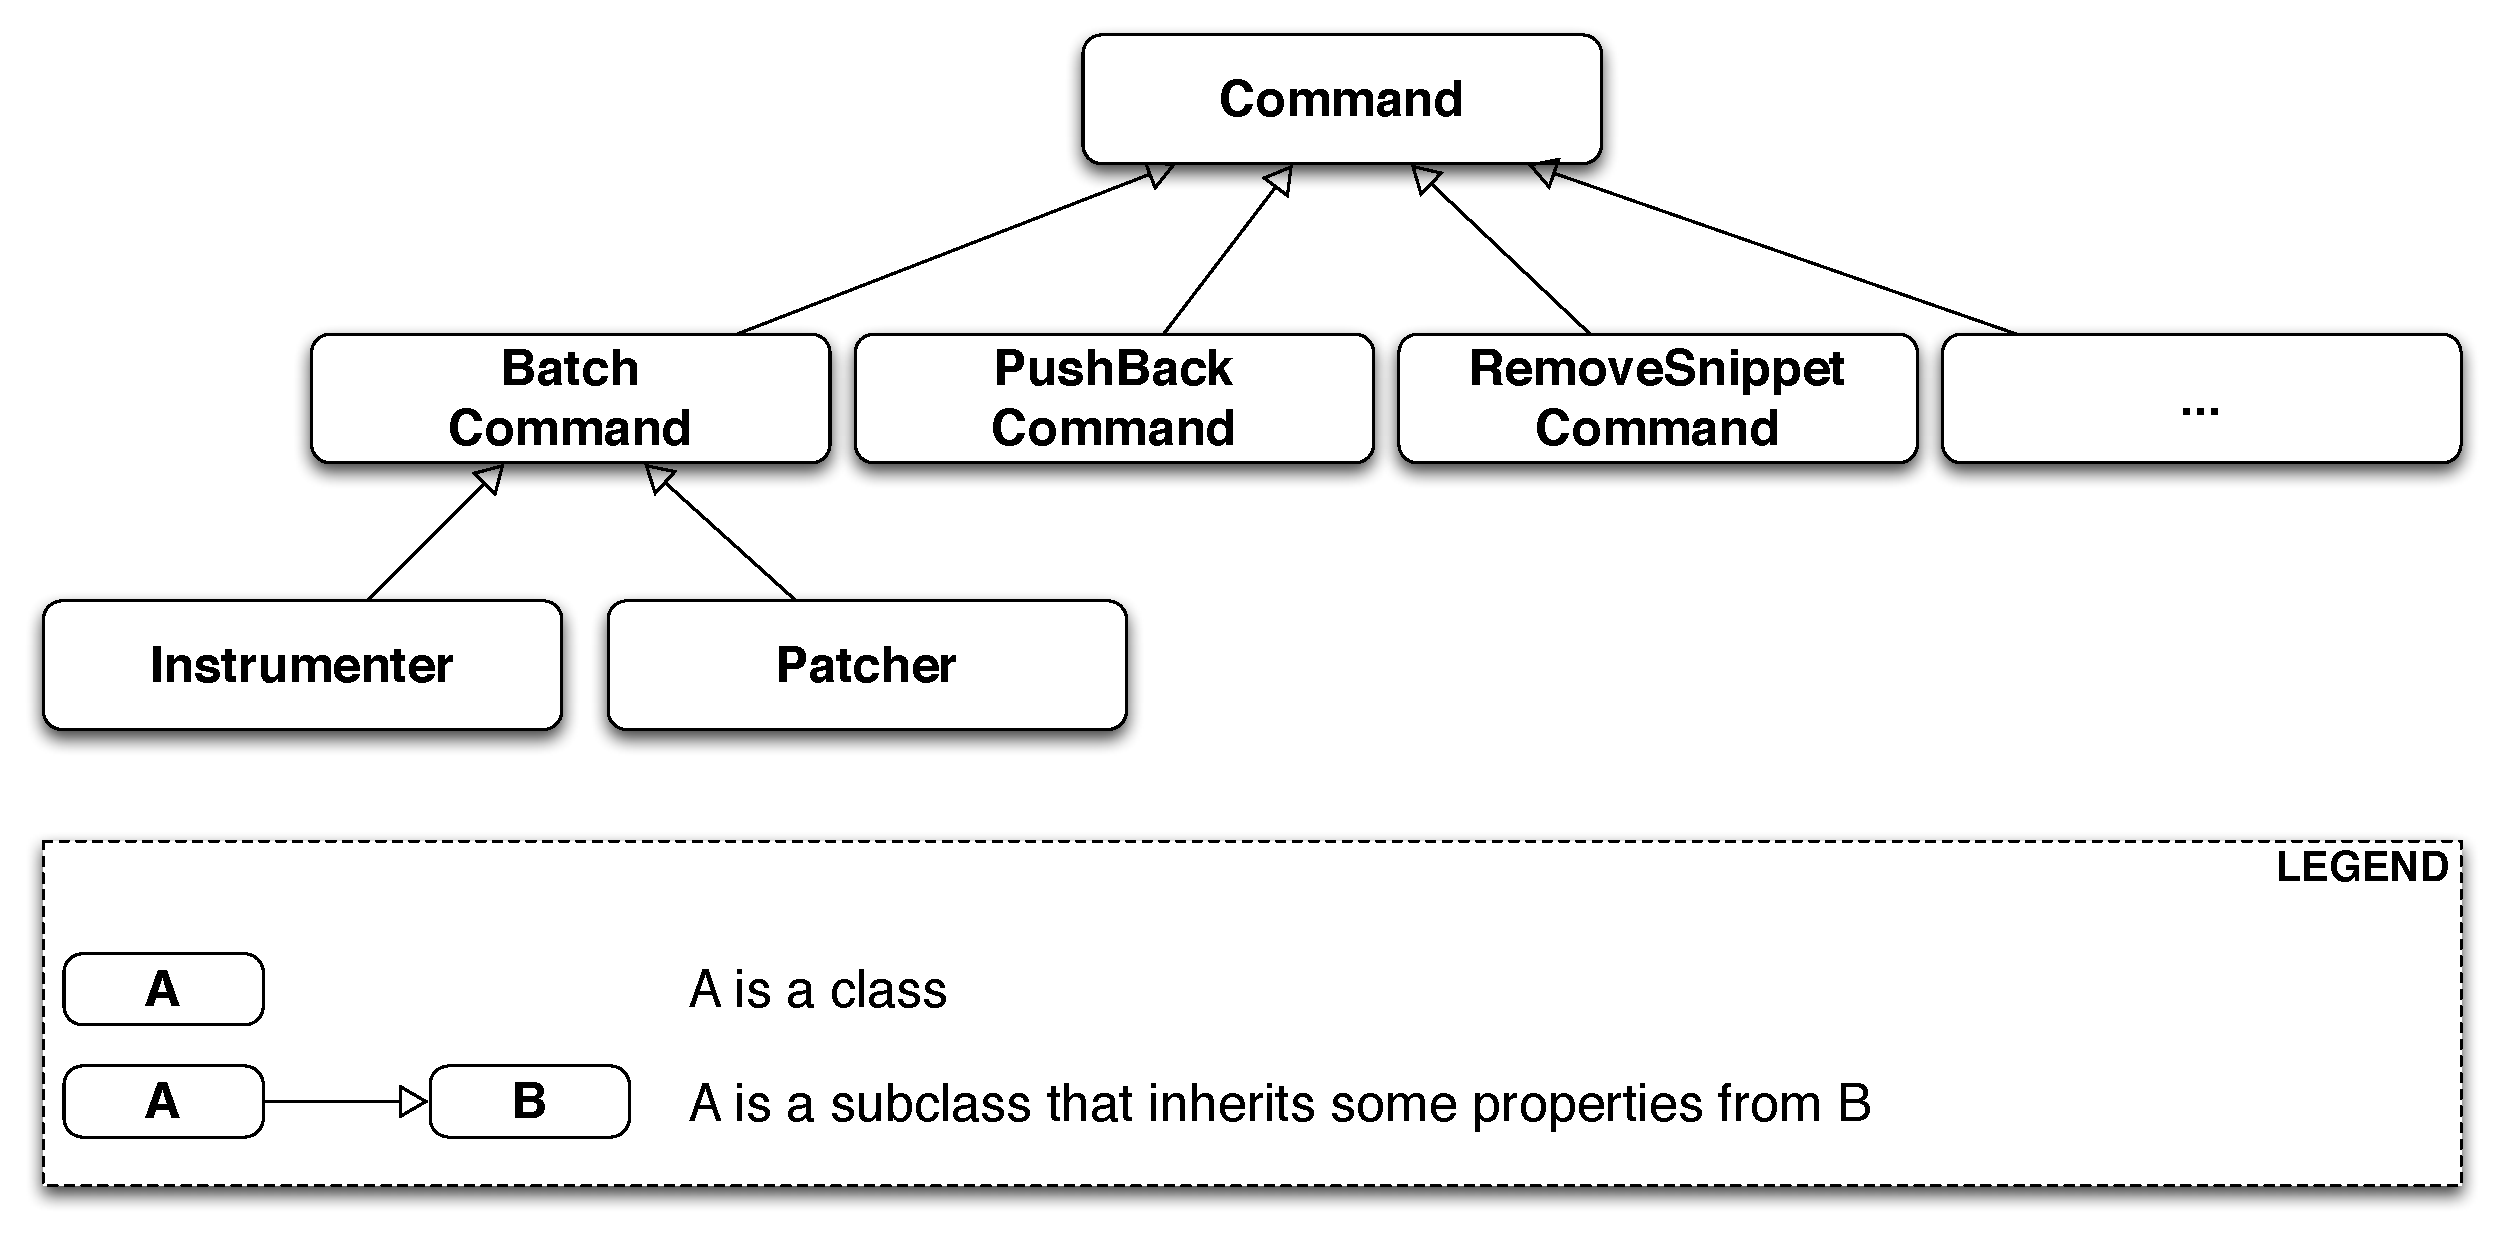
\includegraphics[width=0.85\textwidth]{./figure/command/img.pdf}}
\caption{\label{fig:inh}Inheritance Hierarchy}
\end{figure}


The implementation of an instrumentation engine may be very sophisticated (e.g.,
relocating a function), or be very simple (e.g., simply overwrite an
instruction). Therefore, PatchAPI provides a flexible framework for programmers
to customize the instrumentation engine. This framework is based on Command
Pattern~\footnote{http://en.wikipedia.org/wiki/Command\_pattern}. The
instrumentation engine has transactional semantics, where all instrumentation
requests should succeed or all should fail. In our framework, the
\textbf{Command} abstraction represents an instrumentation request or a logical
step in the code patching process. We accumulate a list of \textbf{Commands},
and execute them one by one. If one \textbf{Command} fails, we undo all finished
\textbf{Commands}. Figure \ref{fig:inh} illustrates the inheritance hierarchy
for related classes. There is a default implementation of instrumentation engine
in PatchAPI for 1st party code patching.
\begin{itemize}
\item \emph{Command} - The Command class represents an instrumentation request (e.g.,
    snippet insertion or removal), or a logical step in the code patching (e.g.,
    install instrumentation). This class provides a run() method and an undo()
    method, where run() will be called for normal execution, and undo() will be
    called for undoing this Command.
\item \emph{BatchCommand} - The BatchCommand class is a subclass of Command, and it is
    in fact a container of a list of Commands to be executed atomically.
\item \emph{Instrumenter} - The Instrumenter class inherits BatchCommand to encapsulate
    the core code patching logic, which includes binary code generation.
    Instrumenter would contain several logical steps that are individual
    Commands.
\item \emph{Patcher} - The Patcher class is also a subclass of BatchCommand. It accepts
    instrumentation requests from users, where these instrumentation requests
    are Commands (e.g., snippet insertion). Furthermore, Patcher implicitly adds
    Instrumenter to the end of the Command list to generate binary code and
    install the instrumentation.
\end{itemize}
